
\section{\rbt}

\vskip0.5cm

\subsection{ROTACIONES}

\begin{center}
		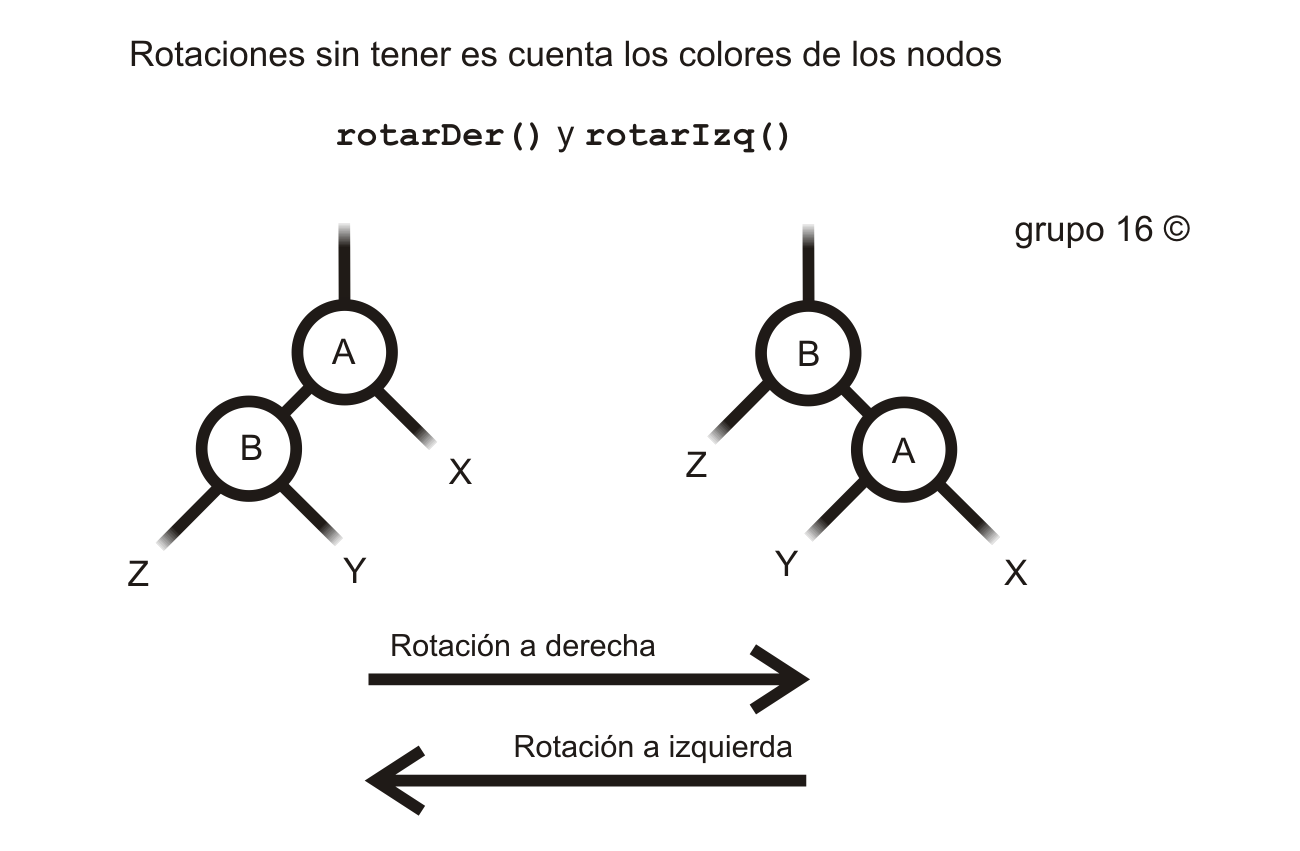
\includegraphics{rotaciones.png} \\
(figura 1.1)\\
\end{center}

Rotaciones simples para mantener el balanceo. (No son para hacerlo un AVL)

\subsection{CASO 1}

\begin{center}
		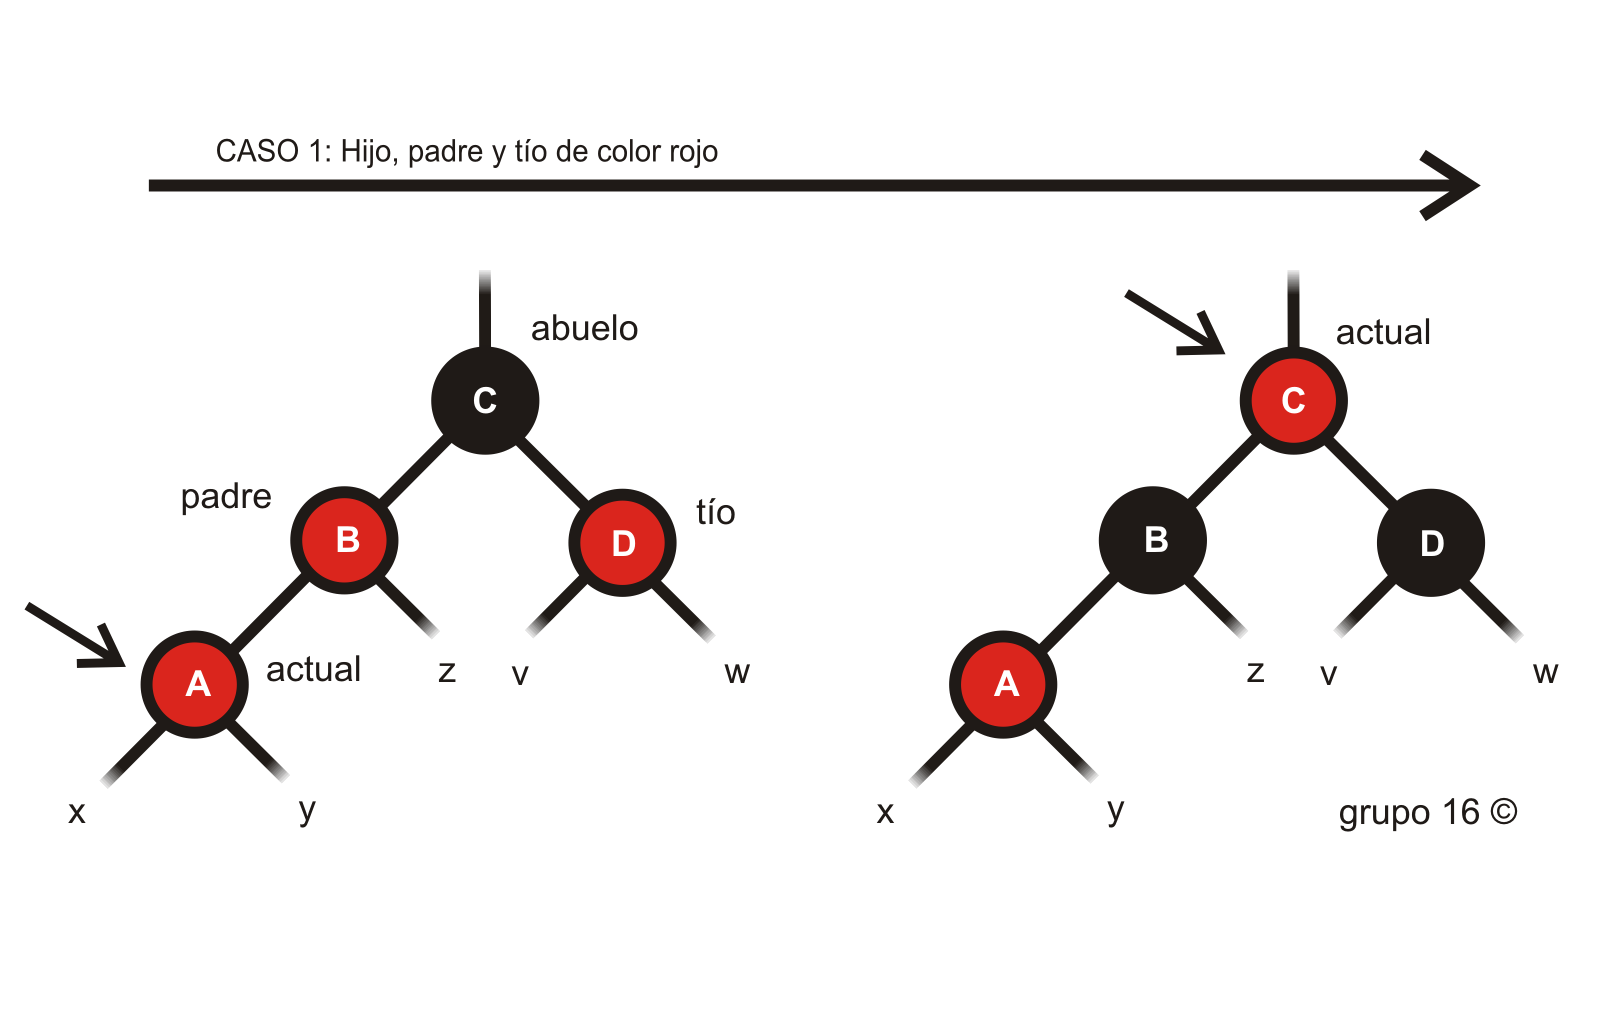
\includegraphics{caso1.png} \\
(figura 1.2)\\
\end{center}

Si A (Actual), B (Padre) y D (tio) son Rojos, estamos en \textsc{CASO 1}.\\
Pintamos al padre y tio de Negro, y pintamos a C (Abuelo) de Rojo. Como el arbol era un \rbt ese abuelo era negro.\\
Al hacer los cambios, alturas negras no se modifican. Por lo que hasta el abuelo tenemos todo arreglado.

\subsection{CASO 2}

\begin{center}
		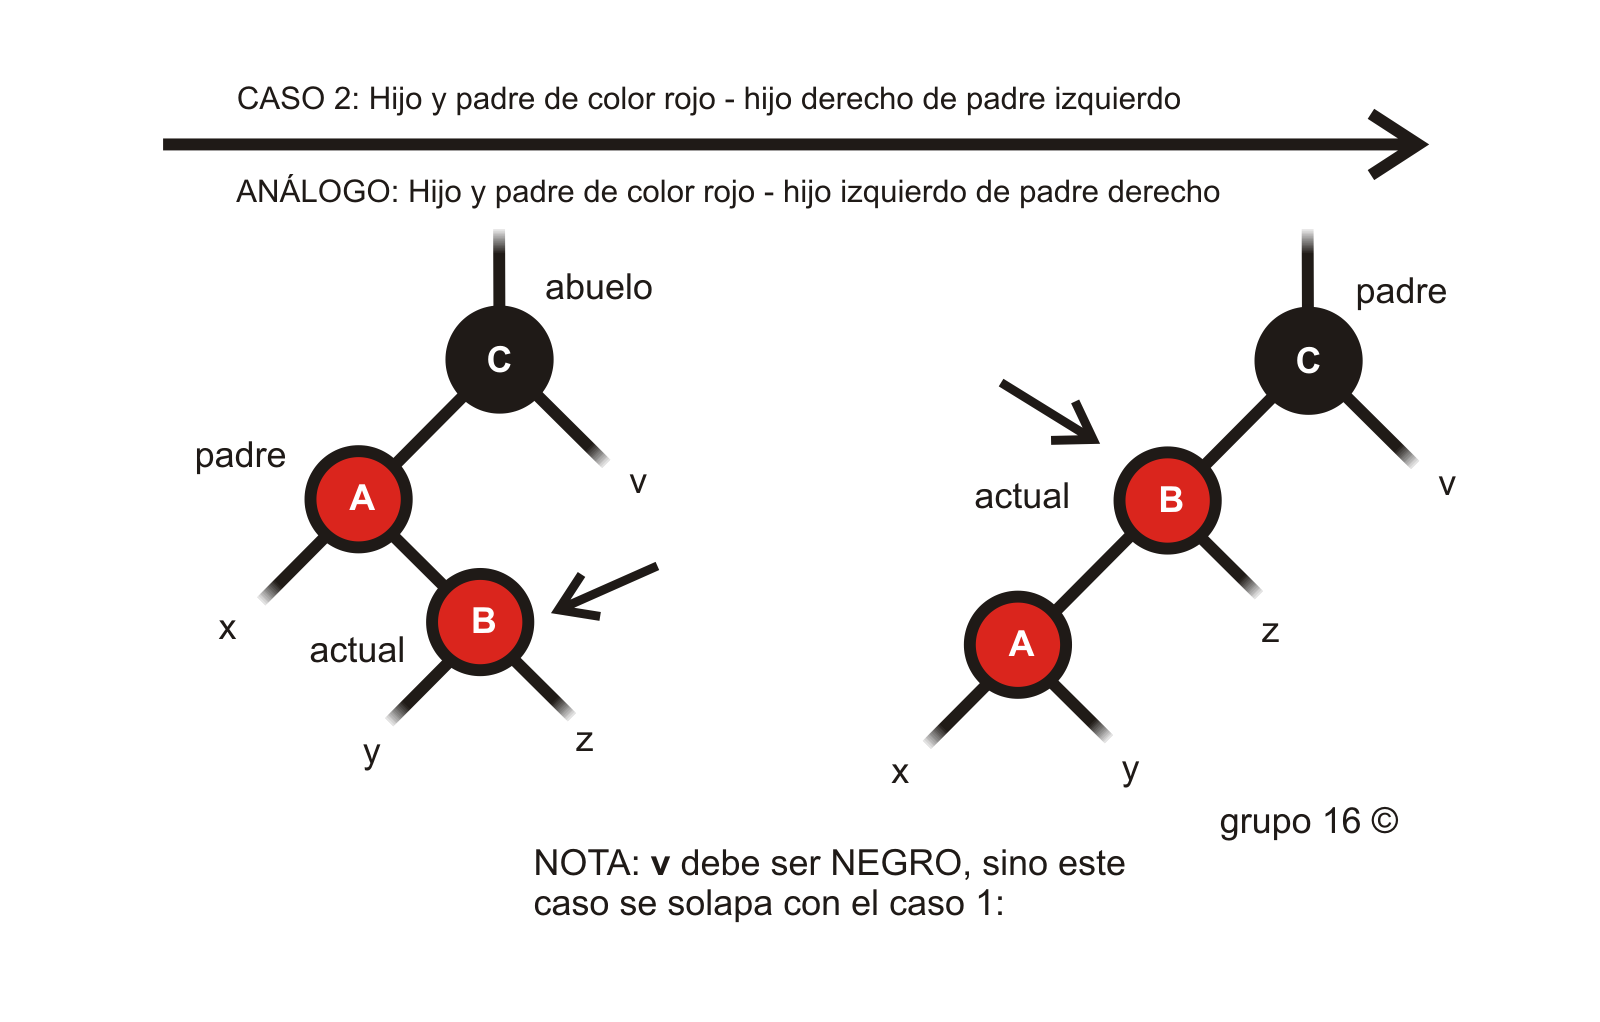
\includegraphics{caso2.png} \\
(figura 1.3)\\
\end{center}

Si B (Actual) y A (padre) son rojos y el tio es negro (o es nil - tambien considerado como regro) y ademas B es hijo derecho de un padre que es hijo izquierdo (o B es hijo izquierdo de un padre que es hijo derecho), estamos en \textsc{CASO 2}\\
Rotamos el padre a izquierda (o derecha segun el caso), y hemos reducido el \textsc{CASO 2} o un \textsc{CASO 3}.

\subsection{CASO 3}

\begin{center}
		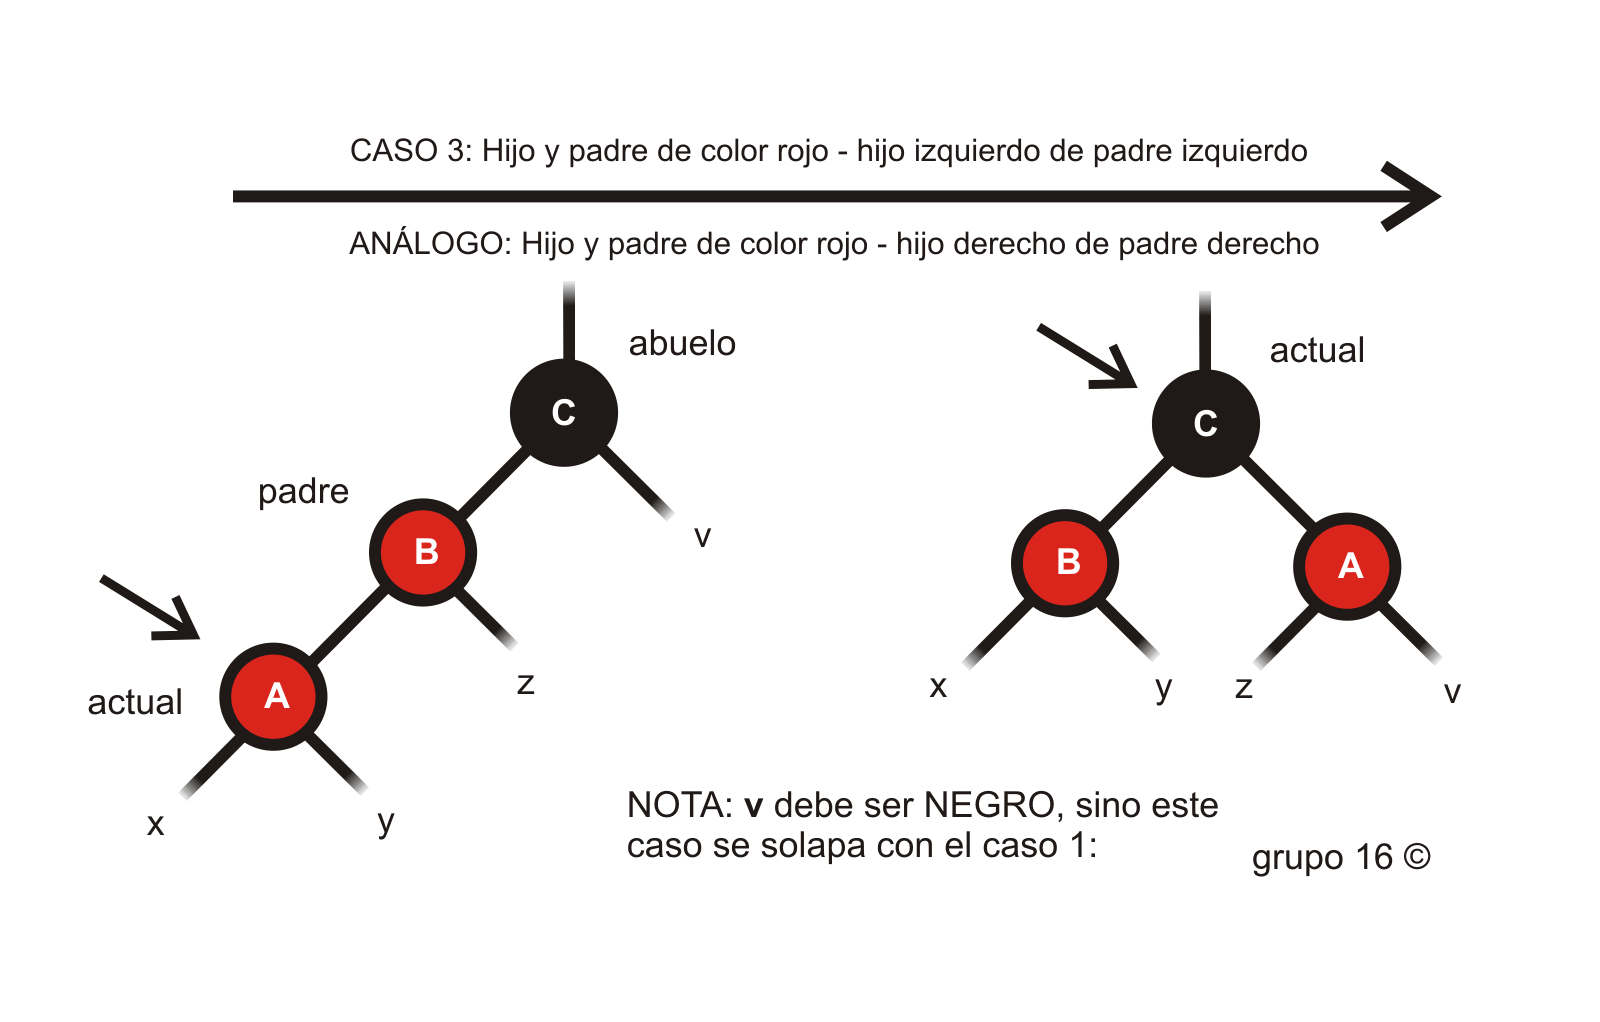
\includegraphics{caso3.png} \\
(figura 1.4)\\
\end{center}

Si A (Actual) y B (padre) son rojos y el tio es negro (o es nil - tambien considerado como regro) y ademas B es hijo derecho de un padre que es hijo derecho (o B es hijo izquierdo de un padre que es hijo izquierdo), estamos en \textsc{CASO 3}\\
Pintamos a padre negro, al abuelo rojo y y rotamos a derecha (o Izquerda segun el caso) al abuelo\\
Las alturas negras no se modifican y la posici�n del abuelo quedar�a negra, con ambos hijos rojo.

\subsection{TEST de Inserciones}

Hemos realizado un par de test para ``verificar'' el correcto fuincionemiento de las inserciones en el \rbt\\
Las inserciones fueron las siguientes $[10, 20, 15, 30, 40]$.\\
De esta manera probamos los casos mas interesantes:

\vskip0.3cm

\begin{tabular}{lll}
de $ninguno$ &			 a $[10]$ 					&	(CASO 0: Insertar raiz)\\
de $[10]$ &				 a $[10, 20]$				&	(CASO 0: Insertar con padres negro)\\
de $[10, 20]$ &			 a $[10, 20, 15]$ 			&	(CASO 2)\\
de $[10, 20, 15]$ &		 a $[10, 20, 15, 30]$ 		&	(CASO 1)\\
de $[10, 20, 15, 30]$ &	 a $[10, 20, 15, 30, 40]$ 	&	(CASO 3)\\
\end{tabular}
                                                                            
\vskip0.3cm

N�tese que en algunas de estas inserciones, \\
los llamados recursivos, llaman tambien a otros casos de ``reacomodacion''.\\
Para correr el test y observar la salida del programa se debe llamar al \verb|main| con parametro \verb|test|

\begin{center}
		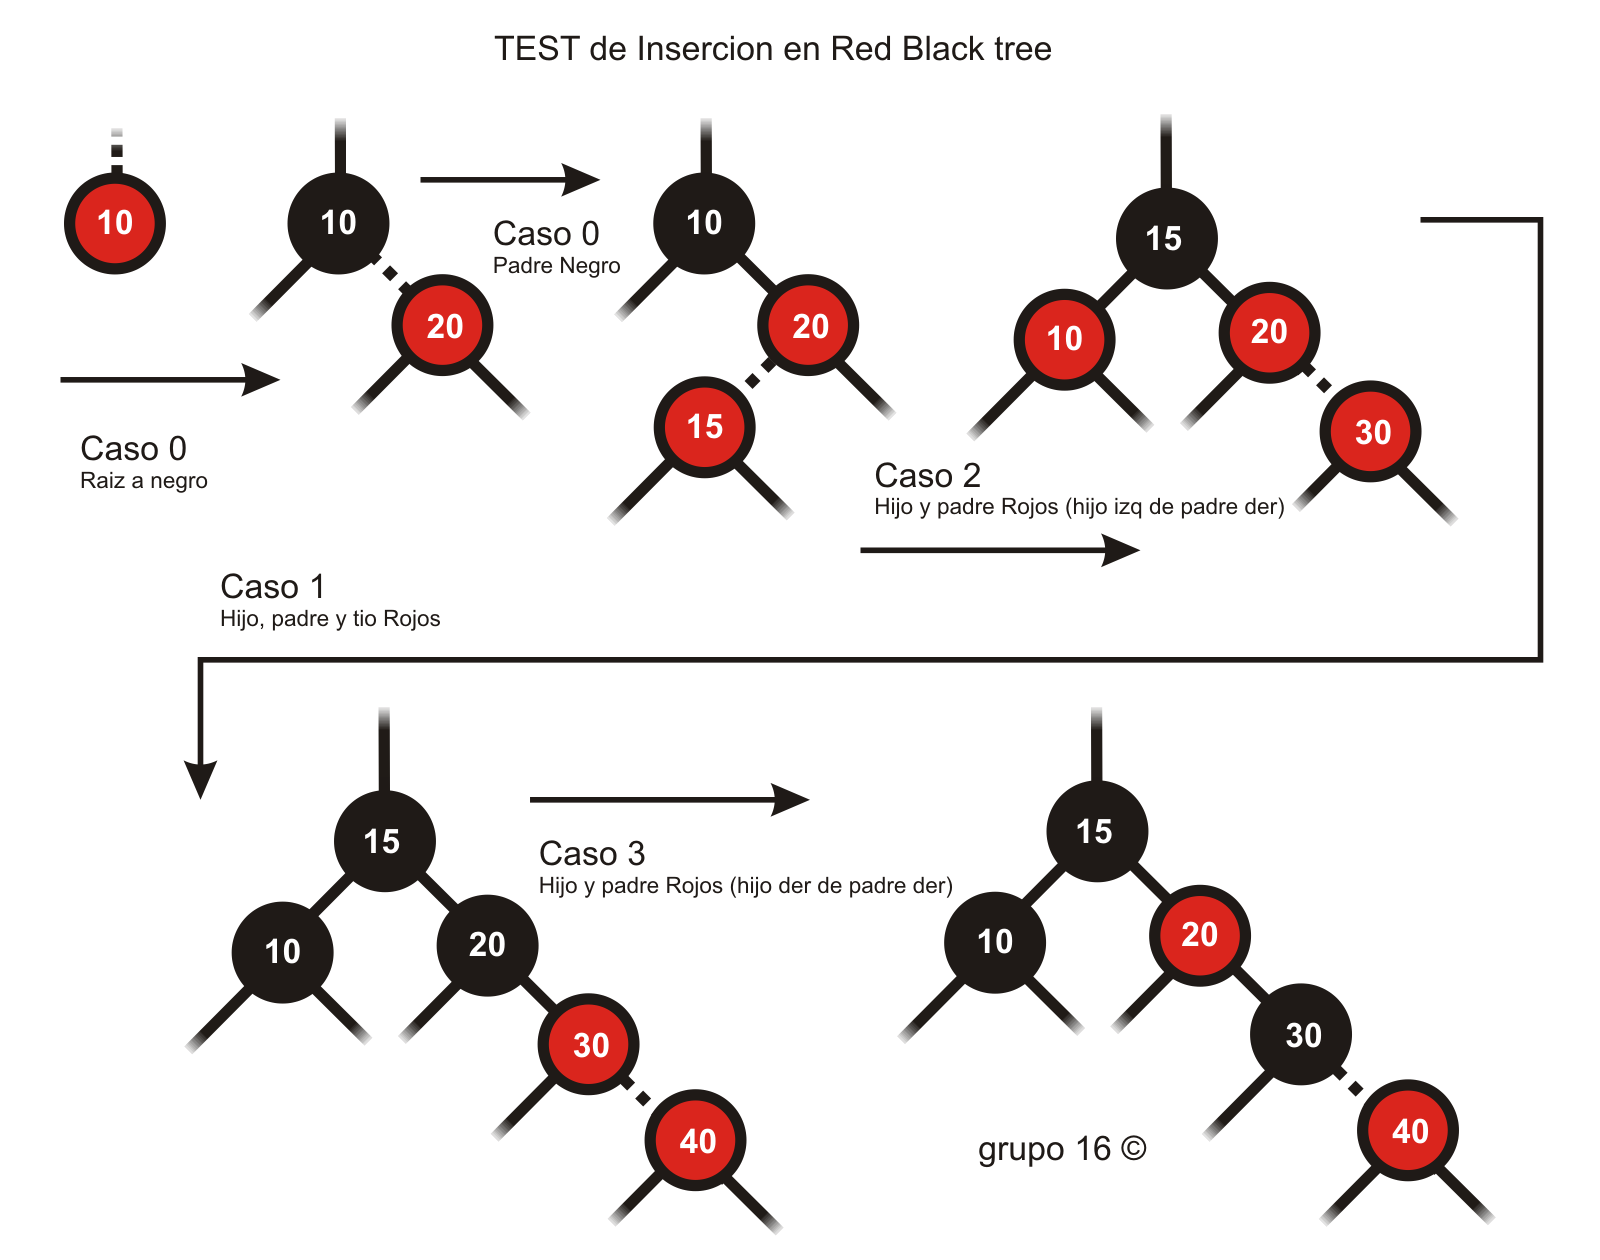
\includegraphics{test_insercion.png} \\
(figura 1.5)\\
\end{center}

\vskip0.5cm




\begin{itemize}
\item \textit{prepararArregloEstanImagenes(int im)}

inicializa un arreglo en false\\
Costo $O(im)$

\item \textit{intervalosElementales(Lista(imagenes) img) $->$ Conj(puntos):res}

\begin{framed}
\begin{verbatimtab}[4]
intervalosElementales(Lista(imagenes) img) -> Conj(puntos):res
{
	desde 0 a Tam(img) hacer	// O(1) / itera im veces
	{
		res <- agregar(x_0)		// O(log(2im))
		res <- agregar(x_1)		// O(log(2im))
	}
	return res					// O(1)
}
\end{verbatimtab}
\end{framed}
Como ingresamos dos puntos por imagen a lo sumo el conjunto tendra $2im$, por lo que pudimos acotar la insercion $log(2im)$.\\
El costo total de este algoritmo es pues $O(im*log(im))$
            
\item \textit{insertar(IntervaloElemental ie)}

\begin{framed}
\begin{verbatimtab}[4]
insertar(IntervaloElemental ie)
{
       ArbolRojoNegro.insertar(ie);
}
\end{verbatimtab}
\end{framed}
Insertar llama a la funcion insertar de \rbt que se va a encargar de insertarlo y ademas de re-establecer el arbol como Red-Black aplicando rotaciones.

\begin{framed}
\begin{verbatimtab}[4]
insertar(T dato)
{
       Nodo actual(dato);        // nodo con el elemento a ingresar
       insertarABB(actual);      // lo inserto de la forma usual en un ABB

       Mientras (No haya reacomodado hasta la raiz y si el padre es rojo)
       {
               Si (el padre del actual nodo es hijo izquierdo)
               {
                       //Me quedo con el tio
                       Nodo tio = hijo izquierdo;

                       Si El tio es Rojo Entonces
                       {       ESTAMOS EN EL CASO 1    }
                       Sino Es Negro
                       {
                               Si actual es hijo derecho del padre
                               {
                                       { ESTAMOS EN EL CASO 2 }
                               // hemos reducido del caso 2 al 3
                               }
                                       { ESTAMOS EN EL CASO 3 }

                       }

               }Sino
               {
                       Si el padre de actual es hijo derecho
                       {
                               // me quedo con la tia
                               Nodo tia = Nodo Izquierdo;

                               Si La tia es Roja Entonces
                               {       ESTAMOS EN EL CASO 1    }
                               Sino Es Negra
                               {
                                       Si actual es hijo izquierdo del padre
                                       {
                                               { ESTAMOS EN EL CASO 2 }
                                       // hemos reducido del caso 2 al 3
                                       }
                                               { ESTAMOS EN EL CASO 3 }
                               }
                       }
               }
       Raiz.Color = Negro; //Ponemos la raiz en Negro

       }
}
\end{verbatimtab}
\end{framed}
En esta funcion utilizamos insertarABB que nos inserta un nodo en el arbol de la forma tradicional, que sabemos que tarda log(n).

Luego tenemos un ``mientras'' que va a iterar hasta que el padre sea Rojo y no haya llegado hasta la raiz. Esto es, en peor caso, recorer el arbol desde el lugar donde insertamos el nodo hasta la raiz. Esto seria ir recorriendo lo ya recorrido pero para arriba. Adem�s cada paso realiza rotaciones y cambios de datos que son O(1). \\
Entonces Complejidad Total en peor caso ser�a: $O(log(n) $(ida-insercionABB)$ + log(n) $(vuelta hasta la raiz)$) = O(log(n))$

\item \textit{llenarIntervalosElementales(Lista(Imagen):imagenes, bool:X)}
\begin{framed}
\begin{verbatimtab}[4]          
llenarIntervalosElementales(Lista(Imagen):imagenes, bool:X)
{
	Conj(IntervaloElemental):puntos = intervalosElementales(imagenes, X);	
										// O(im*log(im))

	por cada punto de "puntos"		// itera im veces
		insertar(punto)				// O(log(n))
}
\end{verbatimtab}
\end{framed}

Entonces la complejidad de insertar todos los intervalos elementales es\\
$O(im*log(im)) + O(im*log(n))$
            
\item \textit{insertarImagen(indice\_img, inicio, final, minimo, maximo, Nodo actual)}
\begin{framed}
\begin{verbatimtab}[4]
insertarImagen(indice_img, inicio, final, minimo, maximo, Nodo actual)
{
	// inicio es el comienzo del intervalo que quiero insertar
	// final es el final del intervalo que quiero insertar
	// minimo es el minimo del intervalo actual,
	// maximo es el maximo del intervalo actual, Nodo actual)

	// caso base:
	si el intervalo que quiero insertar es justo donde estoy //O(1)
 		agrego indice_img a la lista de imagenes del nodo actual //O(1)
	
	// caso recursivo:
	sino quiere decir que debo bajar por uno de sus hijos
	{
		//decido si bajo por uno y/o por otro
		
		si comienzo del intervalo < numero del nodo actual  //O(1)
			hago recursi�n siguiendo por el hijo izq
			(reacomodando los parametros de manera adecuada)
						//reacomodar los param es O(1)
		
		si final del intervalo > numero del nodo actual  //O(1)
			hago recursi�n siguiendo por el hijo der
			(reacomodando los parametros de manera adecuada)
						//reacomodar los param es O(1)
	}
}
\end{verbatimtab}
\end{framed}

Es importante destacar que, como todas las imagenes que insetaremos estan constituidas por intervalos elementales que ya est�n en el �rbol, sabemos que hallaremos siempre algun nodo donde colocar cada ``pedacito'' de la imagen.\\
Lo m�ximo que podemos llegar a recorrer por cada pedacito es log(n) (que es la altura del arbol) pues comenzamos por la raiz y a lo sumo seguimos iterando hasta la hoja.

El problema aqu� es que, en general, nuestra imagen no esta compuesta por un solo intervalo elemental, sino por varios

Recursi�n:\\
Podr�amos decir que, en general, la recursi�n se har� m�s veces hacia un s�lo lado (izq o der), pero es importante saber cu�ntas veces nos podr�a pasar que tengamos que seguir hacia ambos lados $-$si fuera posible que para alguna imagen tengamos que ir siempre por los 2 caminos, terminar�amos recorriendo todos los nodos del arbol y esto es O(n)! $-$, entonces buscamos el peor caso...

Veamos:

Estuvimos pensando mucho al respecto, y notamos los siguientes items:
\begin{itemize}
	\item por invariante de \adi, una misma imagen puede estar a lo sumo 2 veces en un mismo nivel del arbol
	\item si en un mismo nivel figura en 2 nodos la imagen, en los niveles superiores debera estar entre medio de estos (a la izquierda del nodo de la derecha y a la derecha del nodo de la izquierda)
\end{itemize}

Con estas observaciones y analizando detalladamente llegamos a la conclusi�n de que la peor disposici�n ser�a la siguiente:

\begin{center}
		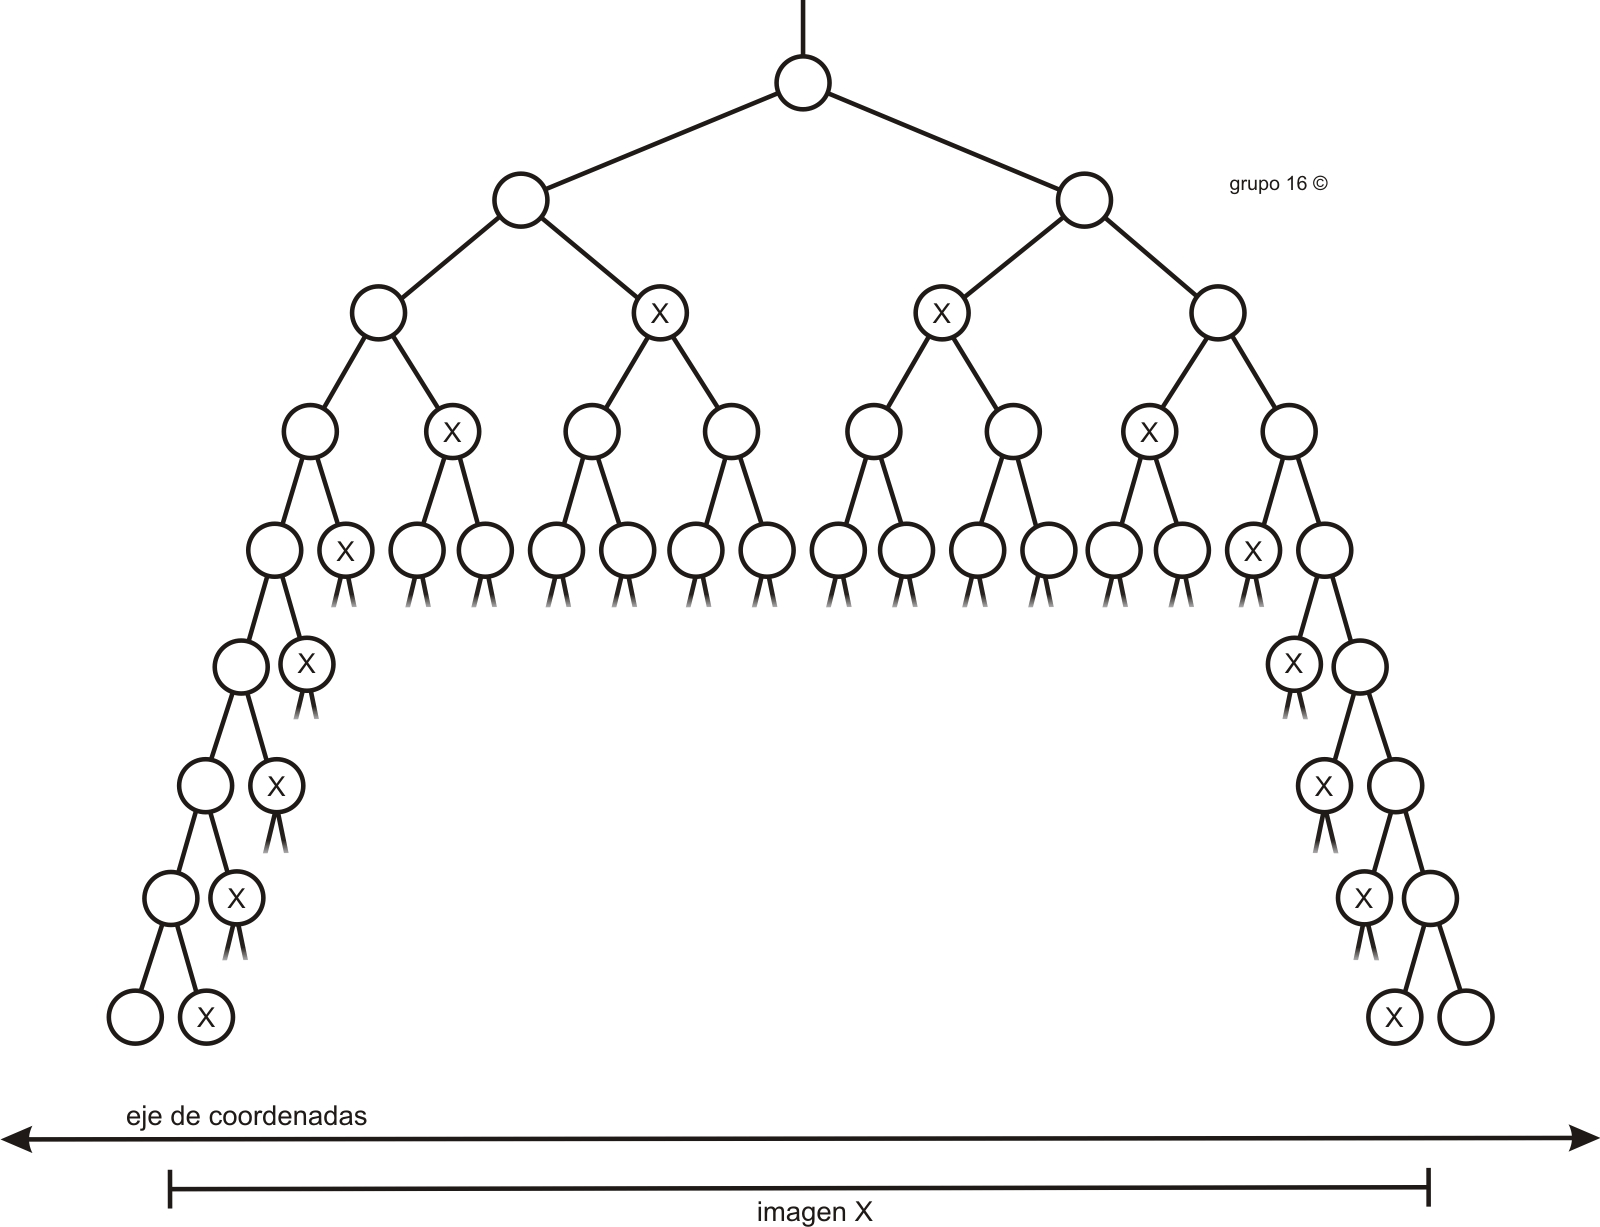
\includegraphics{peorcaso.jpg} \\
(figura 1.5)\\
\end{center}

Como se ve, la imagen X aparece 2 veces en todos los niveles menos en los 2 primeros $-$notar que si apareciera en el primer nivel 
(raiz) no puede estar mas en ningun lugar del arbol, y si apareciera en alguno de los 2 nodos del segundo nivel, entonces ya no 
aparece en ningun nodo mas de esa mitad del arbol.

Y este recorrido es 4*log(n), pues:

\begin{center}
		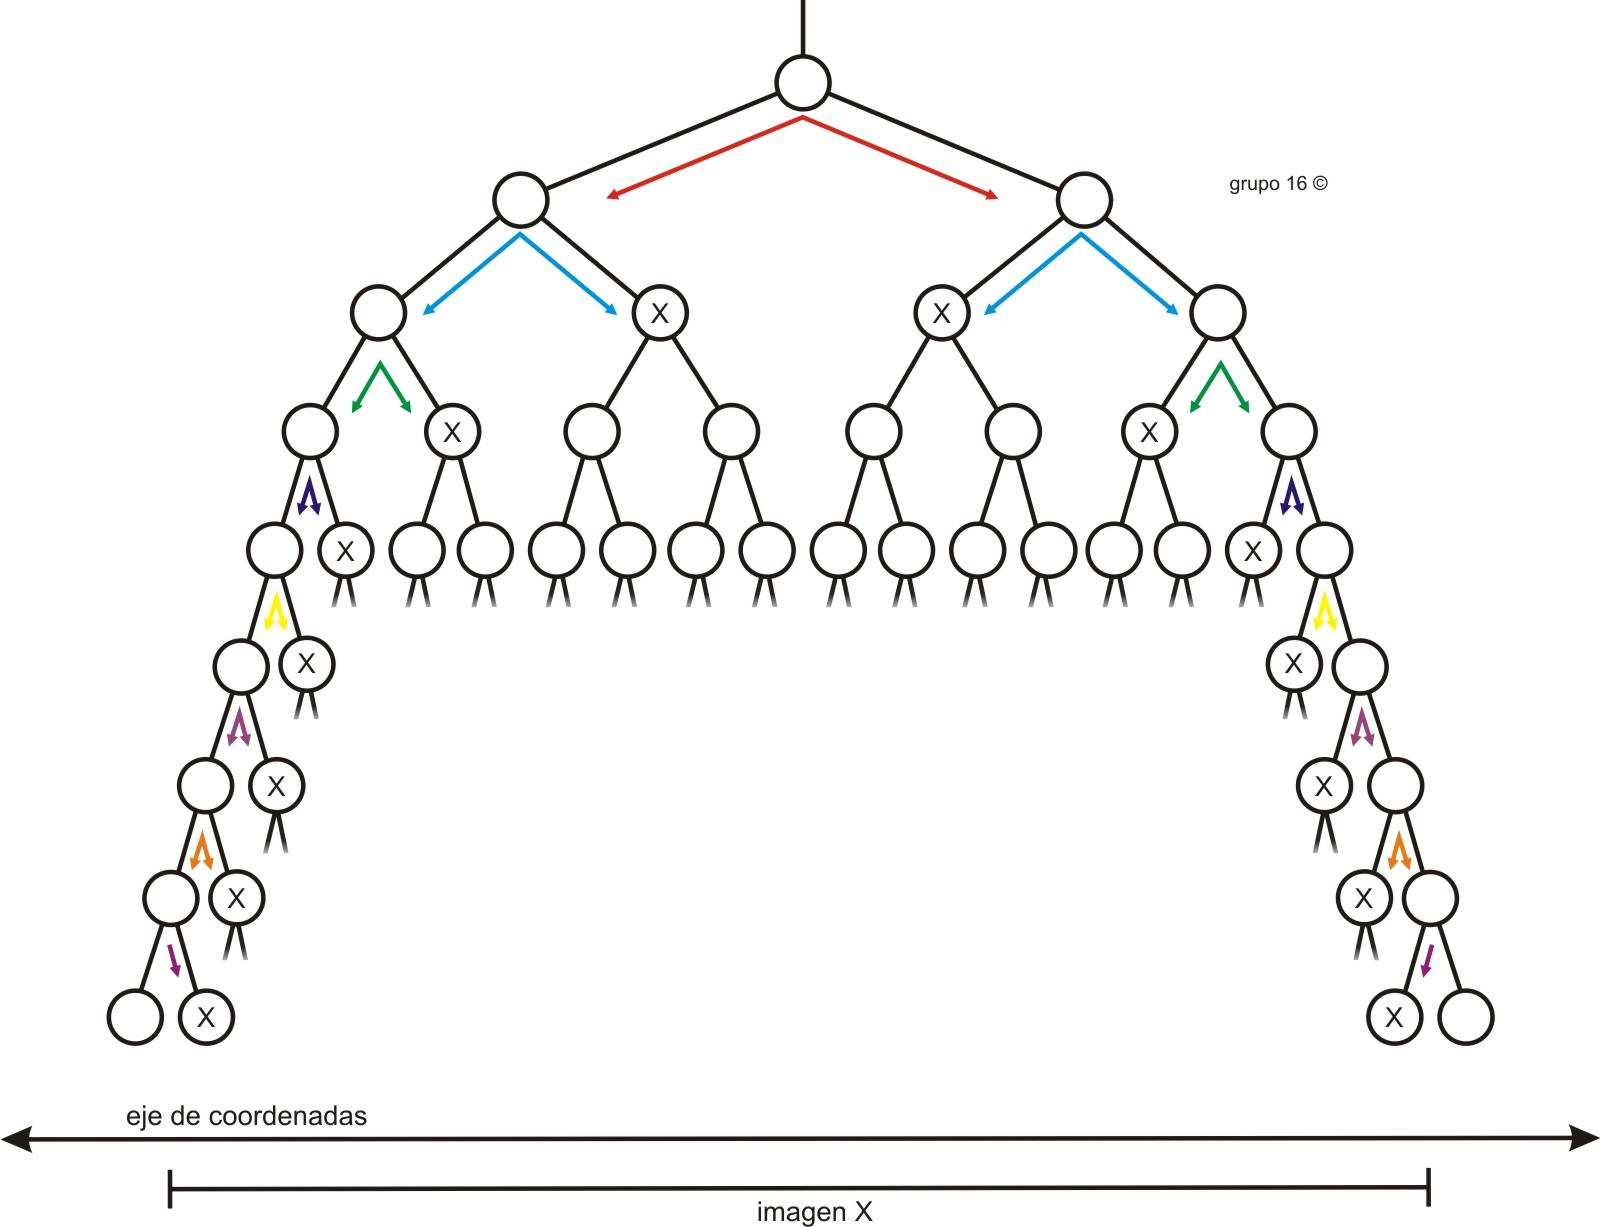
\includegraphics{peorcaso2.jpg} \\
(figura 1.5)\\
\end{center}

La cantidad de ejes recorridos es 2 (primer nivel) + 4 * log(n) (dem�s niveles), y esto es O(log(n)).

Por lo tanto, insertar una imagen en el arbol SIEMPRE tiene cota superior O(log(n)).

      
\item \textit{insertarImagenes(Lista(Imagen):imagenes, bool:X)}
\begin{framed}
\begin{verbatimtab}[4]
insertarImagenes(Lista(Imagen):imagenes, bool:X)
{
	depeniendo de si es por X o por Y
		por cada imagnen de "imagenes"
			insertarImagen(i, inicio, fin, 0, ANCHO_ARBOL, raiz);
}
\end{verbatimtab}
\end{framed}

\item \textit{llenarArbol( Lista(Imagen):imagenes, bool:X) $->$ ArbolDeIntervalos}
\begin{framed}
\begin{verbatimtab}[4]          
llenarArbol( Lista(Imagen):imagenes, bool:X) -> ArbolDeIntervalos
{
	prepararArregloEstanImagenes(im);
	llenarIntervalosElementales(imagenes, X);
	insertarImagenes(imagenes, X);
}
\end{verbatimtab}
\end{framed}




\end{itemize}	

 
            
\begin{itemize}

\item \textit{buscarIndices(int punto, Nodo actual, conj(int))}
\begin{framed}
\begin{verbatimtab}[4]
buscarIndices(int punto, Nodo actual, conj(int))
{
	si no llegue al final del arbol
		res <- agregar(los indices que aparecen en el nodo)
		{
		si  punto es <= actual_numero
			buscarIndices(punto, Izq(actual), conj(int))
		si  punto es >= actual_numero
			buscarIndices(punto, Der(actual), conj(int))		
		}
}
\end{verbatimtab}
\end{framed}

Este es un algoritmo recursivo, que separa siempre el problema es dos partes iguales.\\
�Entra siempre por las dos ramas?... No\\
Existe a lo sumo solo un nodo en el arbol que tiene el mismo valor que el punto buscado, por lo tanto el algoritmo, hace a lo sumo dos caminos.\\
Que recorra uno o dos caminos es despreciable, por lo que su complejidad se puede expresar de la siguinte manera.
\[
\left\{
\displaystyle\matrix{
T(0) = d\hfill\cr
T(n) = T(n/2) + c + k_i
} 
\right.
\]
desarrollando una vez 
\[T(n) = T(n/4) + c + k_i + c + k_j\]
la formula general es
\[T(n) = T(n/2^h) + h*c + \displaystyle\sum_{i=1}^h k_i \]
con $h$ es la altura del arbol\\
como es un \rbt la altura es cercana a $log(n)$
\[T(n) = T(n/2^{log(n)}) + log(n)*c + \displaystyle\sum_{i=1}^h k_i\]
como a cada imagen la incuentro una sola vez por camino (pues si la encontre en un nodo no puedo escontrarla en sus hijos), habr� encontrado al final mis $k$ imagenes buscadas.
\[T(n) = T(n/n) + log(n)*c + k\]
\[T(n) = T(1) + log(n)*c + k\]
Esto da un complejidad total de $O(log(n) + k)$.

\item \textit{busqueda(x, y, Lista(Imagen):Imagenes\_levantadas, bool:X) $->$ Lista(Imagen)}
\begin{framed}
\begin{verbatimtab}[4]
busqueda(x, y, Lista(Imagen):img_levantadas, bool:X) -> Lista(Imagen):res
{
	dependiendo si es por X o por Y					// O(1)
		Lista(int):resIndices;						// O(1)
		buscarIndices(x, raiz, resIndices);			// O(log(n) + k)

		desde i=0 a Tam(resIndices) hacer			// itera k veces
		{			
			si esta entre los valores de y o x		// O(1)
				agregar imagen al resutado			// O(1)
			borrar del vector EstanImagenes			// O(1)
		}		
}
\end{verbatimtab}
\end{framed}

Este algoritmo es simple, consigue los indices de las imagenes que debe agregar segun una de las coordendas ($x$ o $y$) y vesifica luego que cumpla la otra coordenada tambien

Complejidad: $O(2 + log(n) + k + 3k) = O(log(n) + k)$

\end{itemize}